\chapter{Introduction \& Motivation}
\label{introduction}
As networks grow larger and more complex, redundancy becomes desirable and necessary.
Adding redundant links always introduces loops to the network.
Switches and hubs respond to broadcast messages by sending them over every port (except for the one the packet was received on).
This is done in order to ensure every node in the network receives the message.
In conjunction with loops, this behaviour leads to broadcast messages being repeated indefinitely.
With the right network setup, these messages can also multiply exponentially. 
Conditions like this are called broadcast storms\cite{bstorm}.
Figure~\ref{fig:bc_storm} shows how a broadcast storm forms.
In Figure~\ref{fig:bc_storm_a} you can see how Bridge \textit{A} starts the broadcast.
Bridges \textit{B} and \textit{C} then propagate this broadcast over every other port.
This leads to the broadcast being sent in both directions between bridges \textit{B} and \textit{C}, as well as twice along to bridge \textit{D}, as seen in Figure~\ref{fig:bc_storm_b}.
As bridges do not keep messages in memory after they have been sent, they do not recognize broadcast messages they received before.
Thus, they simply propagate the messages in compliance with their policy, leading to the packets multiplying (Figure~\ref{fig:bc_storm_c}).
After the next iteration of propagations the same broadcast message will be sent in both directions over every bridge connection, shown in Figure~\ref{fig:bc_storm_d}.

To prevent this the Spannning Tree Protocol (STP)\cite{perlman85} was created.
It creates an overlay network, in the shape of a tree, to remove loops from the network.
In this overlay, broadcast storms are not possible anymore.
An example for broadcast propagation in an STP overlay network is shown in Figure~\ref{fig:stp_example}.
As shown in Figure~\ref{fig:stp_example}, the overlay ignores the connection between bridges \textit{C} and \textit{D}.
This leads to the broadcast being propagated to every node in just two steps, without any extra packets being generated.

\begin{figure}[p]
    \begin{center}
        \begin{subfigure}[b]{0.4\textwidth}
            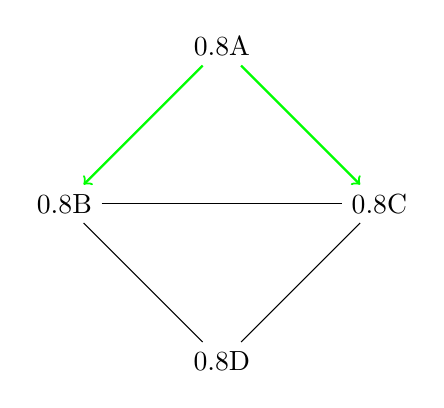
\begin{tikzpicture}
                \node (root) at (4,8) {\switch{0.8}{A}};
                \node (B) at (2,6) {\switch{0.8}{B}};
                \node (C) at (6,6) {\switch{0.8}{C}};
                \node (D) at (4,4) {\switch{0.8}{D}};

                \draw
                (B) edge (C)
                (B) edge (D)
                (C) edge (D);

                \draw[green, thick, ->] 
                (root) edge (B)
                (root) edge (C);
            \end{tikzpicture}
            \caption{Broadcast is sent}
            \label{fig:bc_storm_a}
        \end{subfigure}
        \hspace{1cm}
        \begin{subfigure}[b]{0.4\textwidth}
            \begin{tikzpicture}
                \node (root) at (4,8) {\switch{0.8}{A}};
                \node (B) at (2,6) {\switch{0.8}{B}};
                \node (C) at (6,6) {\switch{0.8}{C}};
                \node (D) at (4,4) {\switch{0.8}{D}};

                \draw 
                (root) edge (B)
                (root) edge (C);

                \draw[green, thick, ->] 
                (B) edge (D)
                (C) edge (D);

                \draw[red, thick, <->]
                (B) edge (C);

                \begin{customlegend}[legend cell align=left, legend entries={Unidirectional Packet, Bidirectional Packet, Connection},
                    legend style={at={(9,9)},font=\footnotesize}]
                    \addlegendimage{green,->}
                    \addlegendimage{red,<->}
                    \addlegendimage{}
                \end{customlegend}
            \end{tikzpicture}
            \caption{Broadcast is propagated}
            \label{fig:bc_storm_b}
        \end{subfigure}
    \end{center}
    
    \begin{center}
        \begin{subfigure}[b]{0.4\textwidth}
            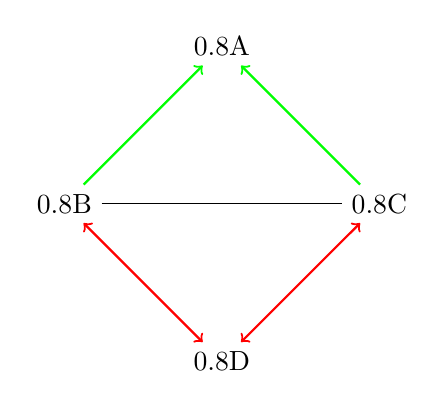
\begin{tikzpicture}
                \node (root) at (4,8) {\switch{0.8}{A}};
                \node (B) at (2,6) {\switch{0.8}{B}};
                \node (C) at (6,6) {\switch{0.8}{C}};
                \node (D) at (4,4) {\switch{0.8}{D}};

                \draw
                (B) edge (C);

                \draw[green, thick, ->]
                (B) edge (root)
                (C) edge (root);

                \draw[red, thick, <->]
                (B) edge (D)
                (C) edge (D);

            \end{tikzpicture}
            \caption{Broadcasts start multiplying}
            \label{fig:bc_storm_c}
        \end{subfigure}
        \hspace{1cm}
        \begin{subfigure}[b]{0.4\textwidth}
            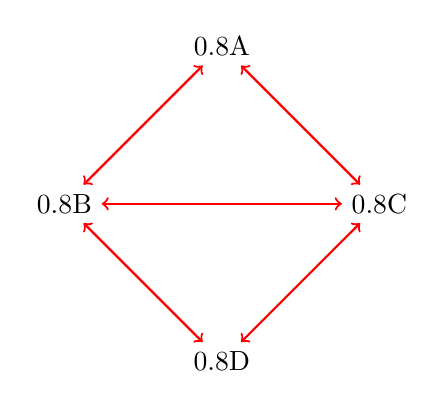
\begin{tikzpicture}
                \node (root) at (4,8) {\switch{0.8}{A}};
                \node (B) at (2,6) {\switch{0.8}{B}};
                \node (C) at (6,6) {\switch{0.8}{C}};
                \node (D) at (4,4) {\switch{0.8}{D}};

                \draw[red, thick, <->]
                (root) edge (B)
                (root) edge (C)
                (B) edge (C)
                (B) edge (D)
                (C) edge (D);
            \end{tikzpicture}
            \caption{Broadcast storm}
            \label{fig:bc_storm_d}
        \end{subfigure}
    \end{center}
    \caption{An example of a broadcast storm}
    \label{fig:bc_storm}
\end{figure}

\begin{figure}[p]
    \begin{centering}
        \begin{subfigure}[b]{0.4\textwidth}
            \begin{tikzpicture}
                \node (root) at (4,8) {\switch{0.8}{A}};
                \node (B) at (2,6) {\switch{0.8}{B}};
                \node (C) at (6,6) {\switch{0.8}{C}};
                \node (D) at (4,4) {\switch{0.8}{D}};

                \draw[green, thick, ->]
                (root) edge (B)
                (root) edge (C);

                \draw
                (B) edge (D);
            \end{tikzpicture}
            \caption{Broadcast is sent}
        \end{subfigure}
        \hspace{1cm}
        \begin{subfigure}[b]{0.4\textwidth}
            \begin{tikzpicture}
                \node (root) at (4,8) {\switch{0.8}{A}};
                \node (B) at (2,6) {\switch{0.8}{B}};
                \node (C) at (6,6) {\switch{0.8}{C}};
                \node (D) at (4,4) {\switch{0.8}{D}};

                \draw[green, thick, ->]
                (B) edge (D);

                \draw
                (root) edge (B)
                (root) edge (C);
                
                \begin{customlegend}[legend cell align=left, legend entries={Unidirectional Packet, Connection},
                    legend style={at={(9,8)},font=\footnotesize}]
                    \addlegendimage{green,->}
                    \addlegendimage{}
                \end{customlegend}

            \end{tikzpicture}
            \caption{Broadcast propagation done}
        \end{subfigure}    
    \end{centering}
    \caption{Broadcast propagation in an STP network}
    \label{fig:stp_example}
\end{figure}

For this thesis, we will only talk about switches.
Hubs, while still existent, are hardly ever used and not STP capable.
We will also refer to switches as bridges, in order to be compliant with STP nomenclature\cite{perlman85}.

Networks with STP utilization are usually quite large.
Additionally, changes and outages are hidden by STP and redundant links in the network.
This can make it hard to keep track of the current network layout.
Debugging STP configurations is also a difficult and time consuming task.
It is possible to check STP configurations via the Simple Network Management Protocol (SNMP).
However, this requires an administrator to connect to every single bridge and collect the STP information manually.
While there are tools to automate this, they rely primarily on SNMP, which may not be supported by all bridges in the network.\\

The aim of this thesis is to create a versatile tool for STP visualization.
We chose to name this tool \textit{\tool}.
\tool\ has the following requirements:
\begin{itemize}
    \item \textbf{STP only}: \tool\ should only rely on STP packets
    \item \textbf{Low traffic}: \tool\ should create as low a traffic as possible
    \item \textbf{Passive}: \tool\ should not provoke any changes in the network and only use packets obtained passively
    \item \textbf{Distributed}: \tool\ is to be run on multiple nodes to send information to a central server where everything is pieced together
    \item \textbf{Low hardware load}: \tool\ should run on simplistic hardware (e.g. a Raspberry Pi) or on a regular PC without slowing it down noticeably
    \item \textbf{No maintenance}: once set up, \tool\ should not require any maintenance (except when updating to a new version)
    \item \textbf{Multiple trees}: if the clients send data from multiple different spanning trees (e.g. one tree per VLAN), these need to be kept seperate.
    \label{requirements}
\end{itemize}

The rest of this thesis is structured as follows: %TODO: rephrase/extend
Chapter~\ref{background} will cover the background knowledge needed to fully understand \tool\ we developed.
In chapter~\ref{stp-gen} we will discuss the implementation and our approach to gathering information from STP packets.
Chapter~\ref{switch} shows the details of our \textit{software-switch} tool, which we had to develop due to problems we encountered with the STP implementations in free router OSs\cite{OpenWrt}\cite{dd-wrt}.
Chapter~\ref{testing} explains how and to what extent we tested \tool, as well as the results.
Finally, Chapter~\ref{conclusion} will summarize this thesis and give an outlook on possible future improvements to \tool.
